%!TEX program = xelatex 
\documentclass{cubeamer}
\usepackage[UTF8]{ctex} % need to use xelatex
\setsansfont{Arial}
\title{Hyperspectral Imaging}
\subtitle{Conference Name}
\author[Longqian Huang]{Polmes \and Longqian Huang} % 
\date{\today} % or whatever the date you are presenting in is
\institute[Zhejiang University]{Optical Science and Engineering}
\copyrightnotice{copyright here}

\begin{document}

\maketitle

\cutoc

\section{Begin a section}
\subsection{Subsection}
\begin{frame}{Frame Title}
	begin a lot of frames
	
    \begin{itemize}
        \item 可以写中文
        \item 去掉ctex宏包将日期换成英文日期
    \end{itemize}
\end{frame}

\begin{frame}{Use columns in a frame}
    \begin{columns}
        \begin{column}{0.6\textwidth}
            \begin{figure}
                \centering
                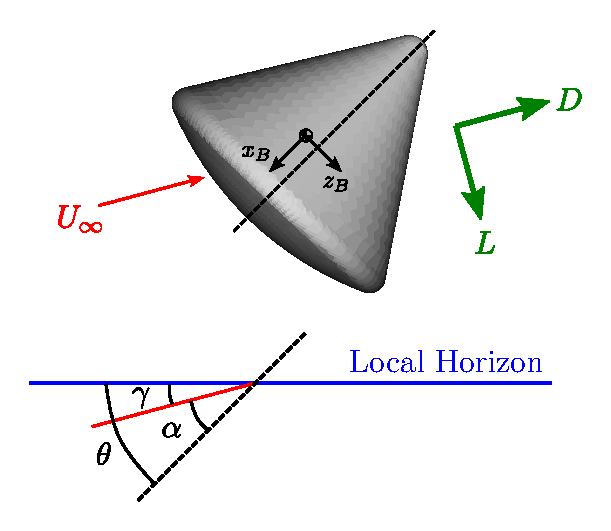
\includegraphics[height = 0.7\textheight]{figures/example.pdf}
                \caption{Fancy Thing from \textit{Source et al.}}
            \end{figure}
        \end{column}
        \begin{column}{0.4\textwidth}
            \begin{itemize}
                \item Some
                \item Interesting
                \item Points
            \end{itemize}
        \end{column}
    \end{columns}
\end{frame}

\section{Interactive section}

\begin{frame}{Make your presentation interactive}
    \begin{cublock}[What about a question to the audience?]
        \begin{overlayarea}{\textwidth}{\baselineskip}
            \only<2->{Followed by the answer.}
        \end{overlayarea}
    \end{cublock}
\end{frame}

% Q&A
\begin{frame}[standout]
    \Huge\textsc{Thank You }
    
    \vfill
    
    \LARGE\textsc{Questions?}
\end{frame}

\section{Notes}
\begin{frame}{notes}
\begin{itemize}
\item 注:原模板来自 CU Boulder Beamer Presentation Template by @polmes
\item 对cls文件简单进行了些修改
\item 会持续更新
\end{itemize}
\end{frame}

\begin{frame}{todos}
\begin{itemize}
\item 搞一个高清好看的反色校徽
\item 进一步美化
\end{itemize}
\end{frame}
\appendix

\begin{frame}{Backup slides go here / Appendix}

    
\end{frame}

\end{document}
